\section{Android security for apps}\label{sect:seapp_andro_sec}

One of the major requirements considered in the design of mobile
operating systems is the need to constrain the ability of apps to
manipulate the execution environment.  Apps may hide functions that
are meant to gain system privileges or capture valuable information
from other apps.  Compared to classical desktop operating systems,
there is greater reliance on the use of apps to access resources or
get services, with more attention paid to limit the ability of apps to
operate in the system.  Advancements in this context can have an
impact on how security for applications is managed in other
domains~\cite{seapp_sok_android}.

\begin{figure}[t]
	\begin{center}
		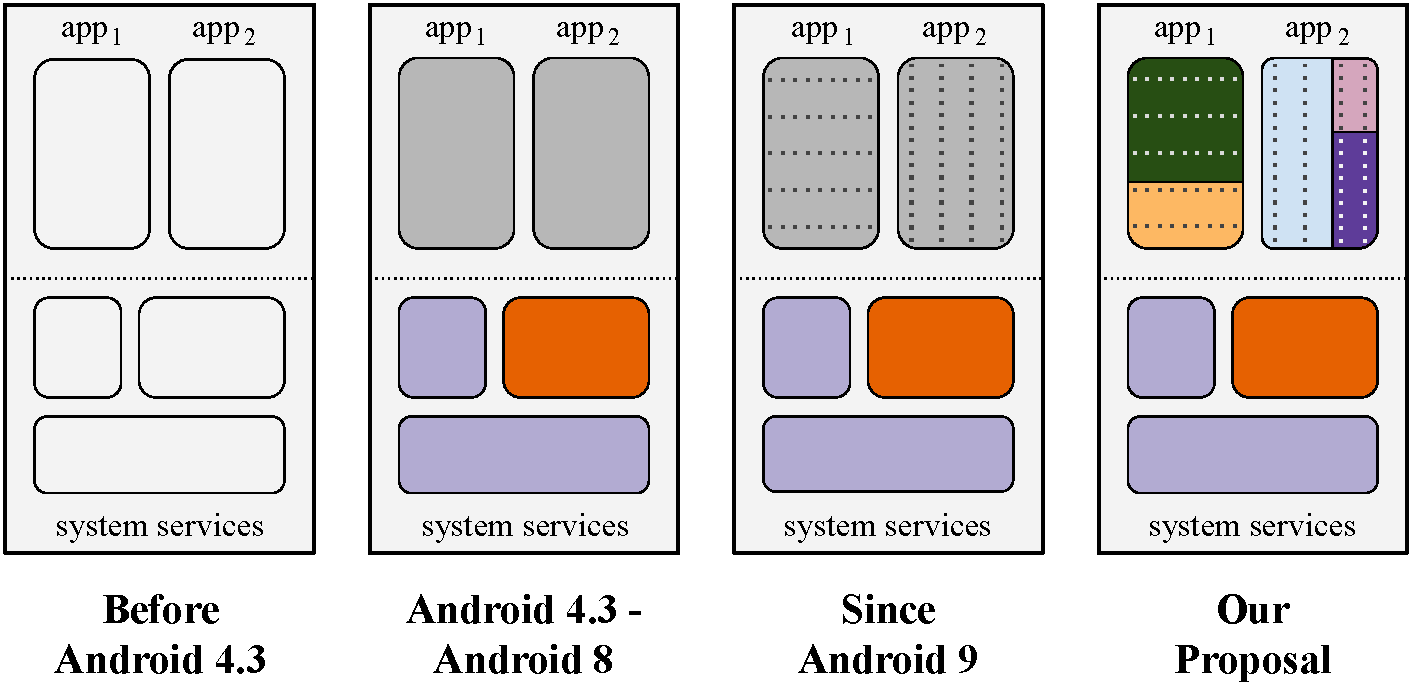
\includegraphics[width=\columnwidth]{chapters/seapp/figs/mac-evolution}
	\end{center}
	\caption[Evolution of the MAC policy in Android]{\label{fig:seapp_mac_evolution} Evolution of the MAC policy
          in Android.  Before 4.3, MAC was not used. Starting with 4.3,
          MAC protects system components. Since 9, categories offer
          rigid MAC protection for apps. Our proposal offers flexible
          MAC protection to apps.}
\end{figure}

The basic principle adopted to manage the threat introduced by apps is
the design of a {\em sandbox}, a restricted environment for app
execution, where anomalous actions by the app are not able to access
resources beyond what has been authorized at app installation time.
The sandbox can be considered a realization of the ``least privilege''
security principle.

The construction of the app sandbox is based on three access control
mechanisms: Android permissions~\cite{seapp_andro_perm,
  seapp_10.1145/2046707.2046779,seapp_10.1145/2335356.2335360},
Discretionary Access Control
(DAC)~\cite{seapp_10.1145/3134600.3134638}, and Mandatory Access
Control (MAC)~\cite{seapp_dacmac}; each of them roughly aligning with
how users, developers, and the platform grant consent, respectively.

Permissions restrict access to sensitive data and services.  In
the \manifest~\cite{seapp_andro_man}, each app statically lists the
Android permissions needed to fully operate.  Not all of them may be
granted; depending on the threat they pose from a security and privacy
standpoint, they may be granted as part of the installation procedure,
or prompted to the user when the app needs them.

DAC restricts access to resources based on user and group identity.
By assigning each application a unique UNIX user ID (UID) and a
dedicated directory, Android isolates apps from each other and from
the system.  However, UID sandboxing has a number of shortcomings.  As
an example, processes running as root are not subject to these
restrictions.  For this reason, when such a process is misbehaving,
for instance due to a bug, it can access private app data files.  DAC
discretionality itself is a problem.  Indeed, as apps and system
processes could override safe defaults, they are more susceptible to
dangerous behavior, such as leaking files or data across security
boundaries via IPC or fork/exec.  Despite its deficiencies, UID
sandboxing is still the primary enforcement mechanism that separates
apps from each other, establishing the foundation upon which further
sandbox restrictions have been built.

MAC dictates which actions are allowed based on the security policy
defined by the system.  Specifically, only actions explicitly granted
by the policy are permitted.  To decide whether to permit or deny an
action, a set of policy rules concerning the {\em security contexts}
(i.e., collections of security labels that classify resources) of the
involved parties is evaluated.

In Android, MAC is implemented using \sea, a set of kernel
modifications part of the Linux Security Module (LSM)
framework~\cite{seapp_lsm_fra}.  Since its first introduction with the
Security Enhanced Android (\sea) project~\cite{seapp_seandroid}, \sel
has been extensively applied to protect system components.  Initially,
it was used to assert the security model requirements during
compatibility testing, then its usage grew further at each release.
In the current version Android 11, \sel is also used to isolate the
rendering of untrusted web content (by the \isolatedapp domain), to
restrict \ioctl system calls~\cite{seapp_restrioctly}, thus limiting
the reachability of potential kernel vulnerabilities, and to support
multi-user separation and app sandboxing with \sel categories.  This
last aspect permits to enforce app separation both at DAC and MAC.
Android dynamically assigns categories to apps during app
installation, so that: (i) an app running on behalf of a user cannot
read or write files created by the same app on behalf of another user
(since Android 6 \cite{seapp_android6_per_user}); and, (ii) an app
cannot read or write files created by another app (since
Android~9\cite{seapp_android9_per_app}).  Before Android~9, this
separation was only enforced at DAC level.  This overlap of security
measures is of extreme relevance to the enforcement of the Android
Security Model and our proposal moves in the same direction.  To
bypass these protections, a process should be granted root
permissions, \dacoverride or \dacreadsearch, and run as SELinux
\mlstrustedsubject; only a few critical system services run in this
configuration.

Android restricts the \sel implementation to the policy enforcement,
ignoring most policy management functions.  The motivation is that the
system policy only changes between releases, therefore support to
runtime changes is not needed.

%%% Local Variables: 
%%% mode: latex
%%% TeX-master: "../../../main.tex"
%%% reftex-default-bibliography: "../../../bib/biblio.bib"
%%% End:
